\chapter{Properties of RIR}
\label{chapter:rir}
This chapter discusses various properties exhibited by RIR. The enhancement algorithms proposed in subsequent chapters incorporate these RIR properties. The time and frequency domain structure of RIR is discussed first. The later part discusses structures present in the RIR magnitude spectrogram. 

\section{Structure of RIR}
This section discusses time domain and frequency domain structure of RIR. 

\subsection{Time domain structure}
The Figure~\ref{fig:rir_time_domain} shows the time domain structure of a recorded RIR available from REVERB challenge database. The RIR has a $T_{60}\approx 700$~ms and source-microphone distance of $2$~m. A similar observations are obtained for other RIRs. The initial part of RIR consists of a short duration of near-zero amplitude that is followed by a peak. This peak represents the speech reaching the microphone due to direct-path propagation. Minimum energy loss occurs in direct-path propagation since it does not undergo absorption due to reflections from the walls. Hence this peak has a high amplitude. The near-zero amplitude region occurring before the peak amplitude corresponds to the direct-path propagation delay. The direct-path peak is followed by other peaks that correspond to the reflected paths. The peaks occurring near the direct-path peak occur due to the strong reflections from the walls. These peaks have relatively larger values when compared with later reflections. The overall structure of the RIR magnitude decays with time.  

The reverberant part of RIR is divided into two regions - early and the late reflections~\cite{naylor2010speech}. Such a distinction is made because of the unique effects caused by these regions on the clean speech. The reflections reaching the microphone with a delay of up to $50$~ms after the direct path from the early reflections. The reflections reaching after $50$~ms forms the late reverberation (reverberation tail). The early reflections are constituted by well-defined reflections and have larger amplitudes. 
The early refection mostly causes spectral changes to clean speech. This perceptual effect is referred to as spectral coloration. Early reflections are indistinguishable from direct-path sound due to the temporal masking of ears. This effect has shown to improve speech intelligibility. However, coloration degrades the quality of recorded speech~\cite{naylor2010speech,kuttruff2016room}. Reverberation tail has smaller amplitudes and diffused nature i.e., sound comes from all directions. The reverberation tail can extend for a longer duration and it gives a perception of sound 'ringing on' effect for a short duration before the reverberant speech starts decaying. This temporal smearing effect gives the impression of space and distance~\cite{naylor2010speech}. The reverberation tail is a major contributor to degradation in speech quality and deteriorates ASR performance.   
%The early refection mostly causes spectral changes to clean speech. This perceptual effect is referred to as spectral coloration. Early reflections are indistinguishable from direct-path sound due to the temporal masking of ears. This effect has shown to improve speech intelligibility. However, coloration degrades the quality of recorded speech~\cite{naylor2010speech,kuttruff2016room}. Reverberation tail has smaller amplitudes and diffused nature i.e., sound comes from all directions. The reverberation tail can extend for longer duration. It is a major contributor for degradation in speech quality and deteriorate ASR performance.  
\begin{figure}[ht!]
\centering
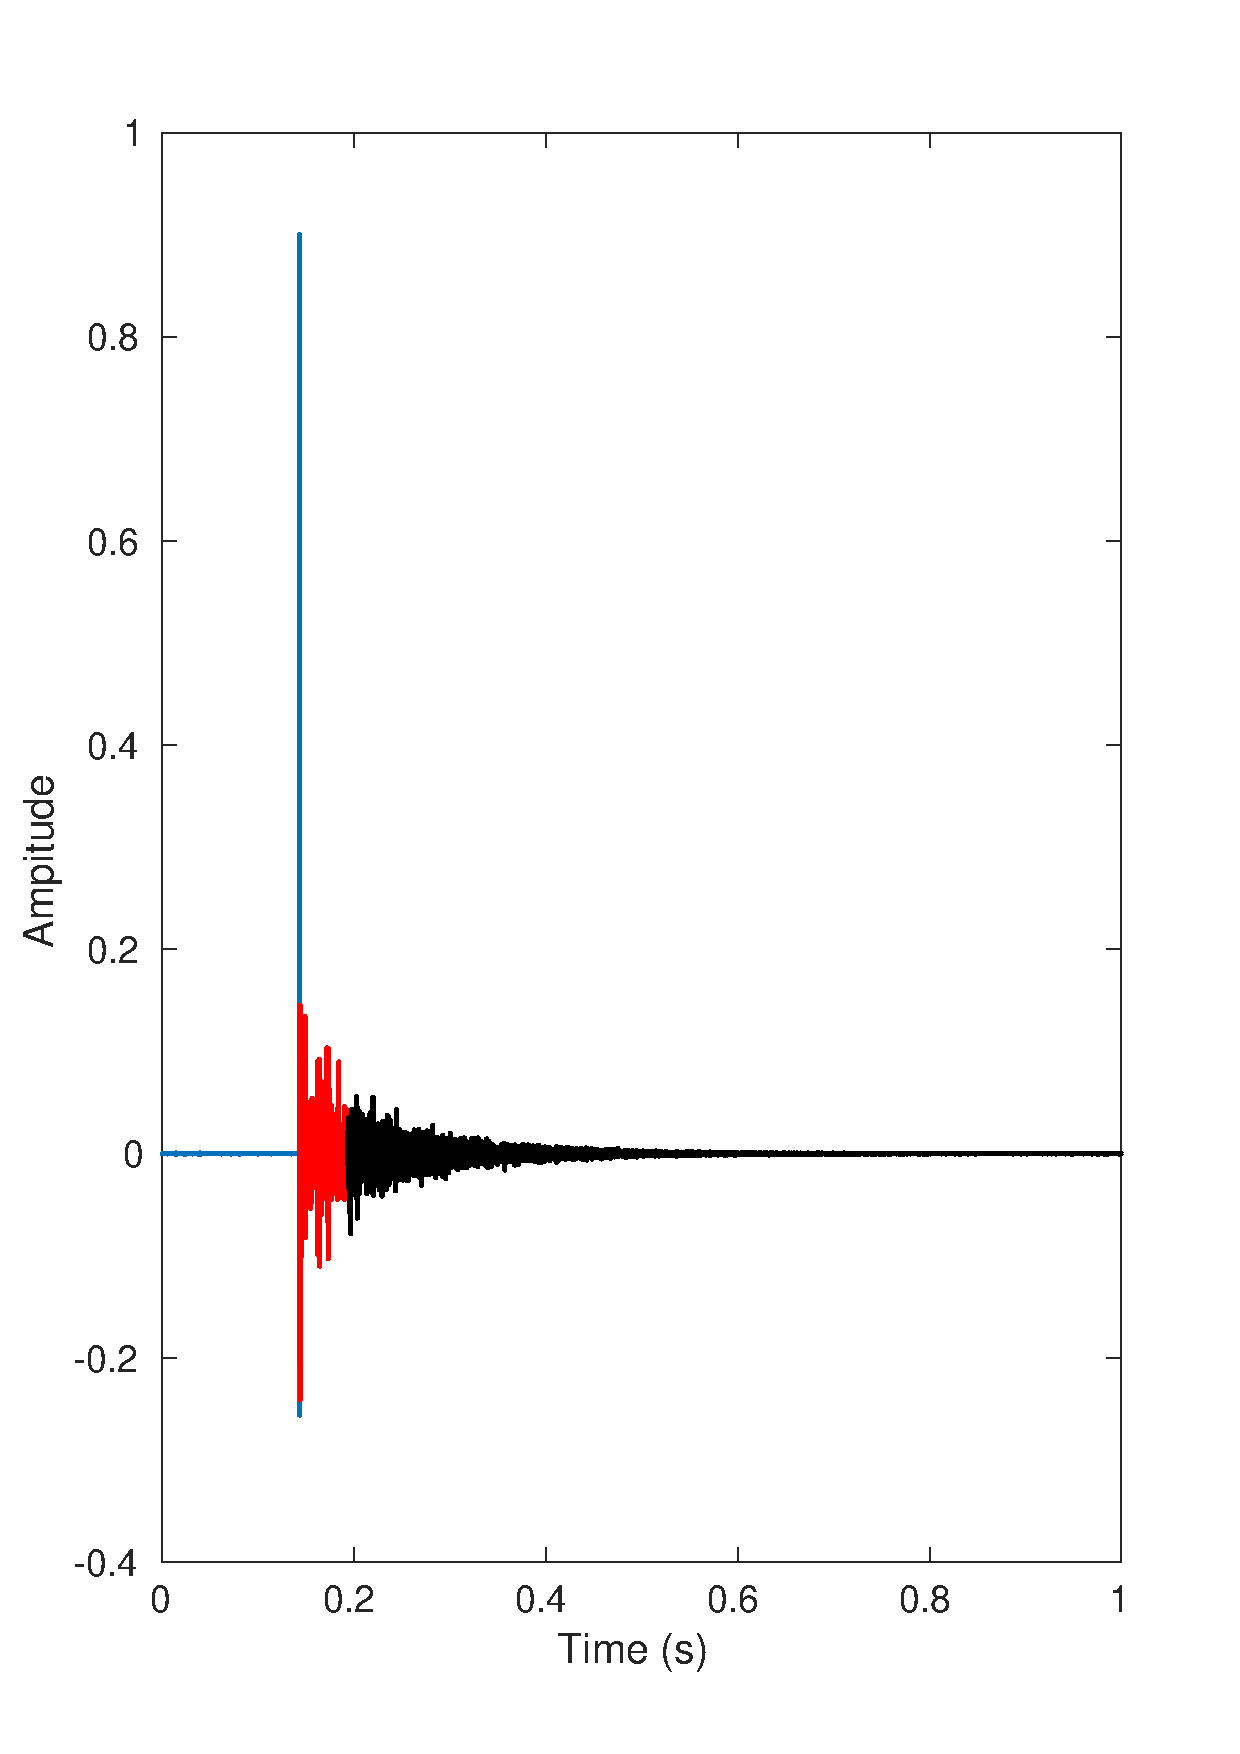
\includegraphics[width=\linewidth]{rir_time_domain.pdf}
\label{fig:rir_time_domain}
\end{figure}

\subsection{Magnitude spectrum of RIR}
The Figure~\ref{fig:rir_spectrum} shows the log-magnitude spectrum for the RIR shown in Figure~\ref{fig:rir_time_domain}. It can be observed that the average difference between spectral maximum and minimum is more than $10$~dB~\cite{kuttruff2016room}. The magnitude spectrum also exhibits spectra null for some frequencies. These effects imposes serious limitations on use of inverse filtering based approaches to compensate for the effects of reverberation.   
\begin{figure}[ht!]
\centering
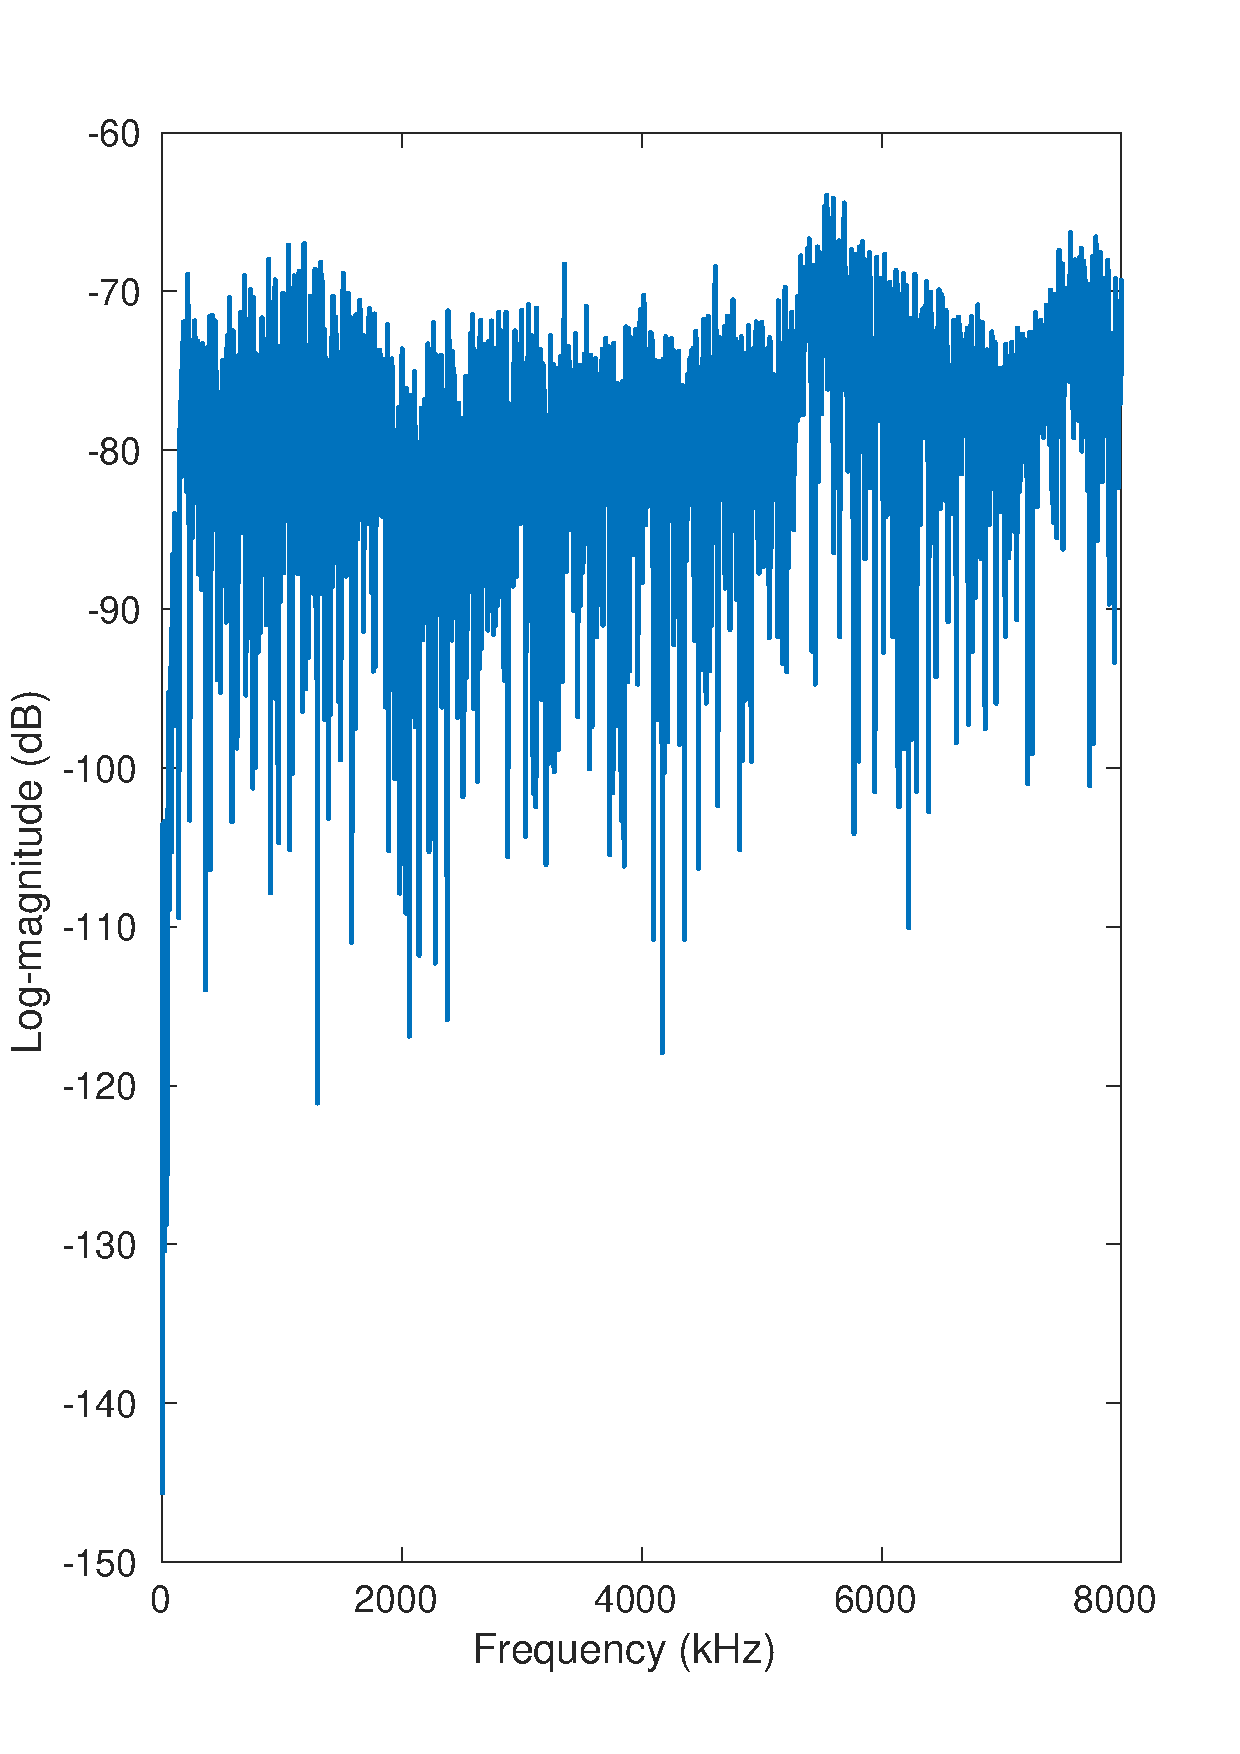
\includegraphics[width=\linewidth]{rir_spectrum.pdf}
\label{fig:rir_spectrum}
\end{figure}

\subsection{Pole-zero plot of RIR}
The Figure~\ref{fig:rir_pole_zero} shows the pole-zero plot for the RIR shown in figure~\ref{fig:rir_time_domain}~\footnote{The multiplicity of poles and zeros are not shown in the plot for simplicty as the non-minimum phase nature of RIR does not change with multiplicity.}. Most of the zeros are located near the unit circle. Out of these zeros, some lie inside the  unit circle while others lie out side the unit circle. This make the RIR a non-minimum phase system. Such an observation is observed for RIRs estimated for most real rooms~\cite{neely1979invertibility}.
\begin{figure}[ht!]
\centering
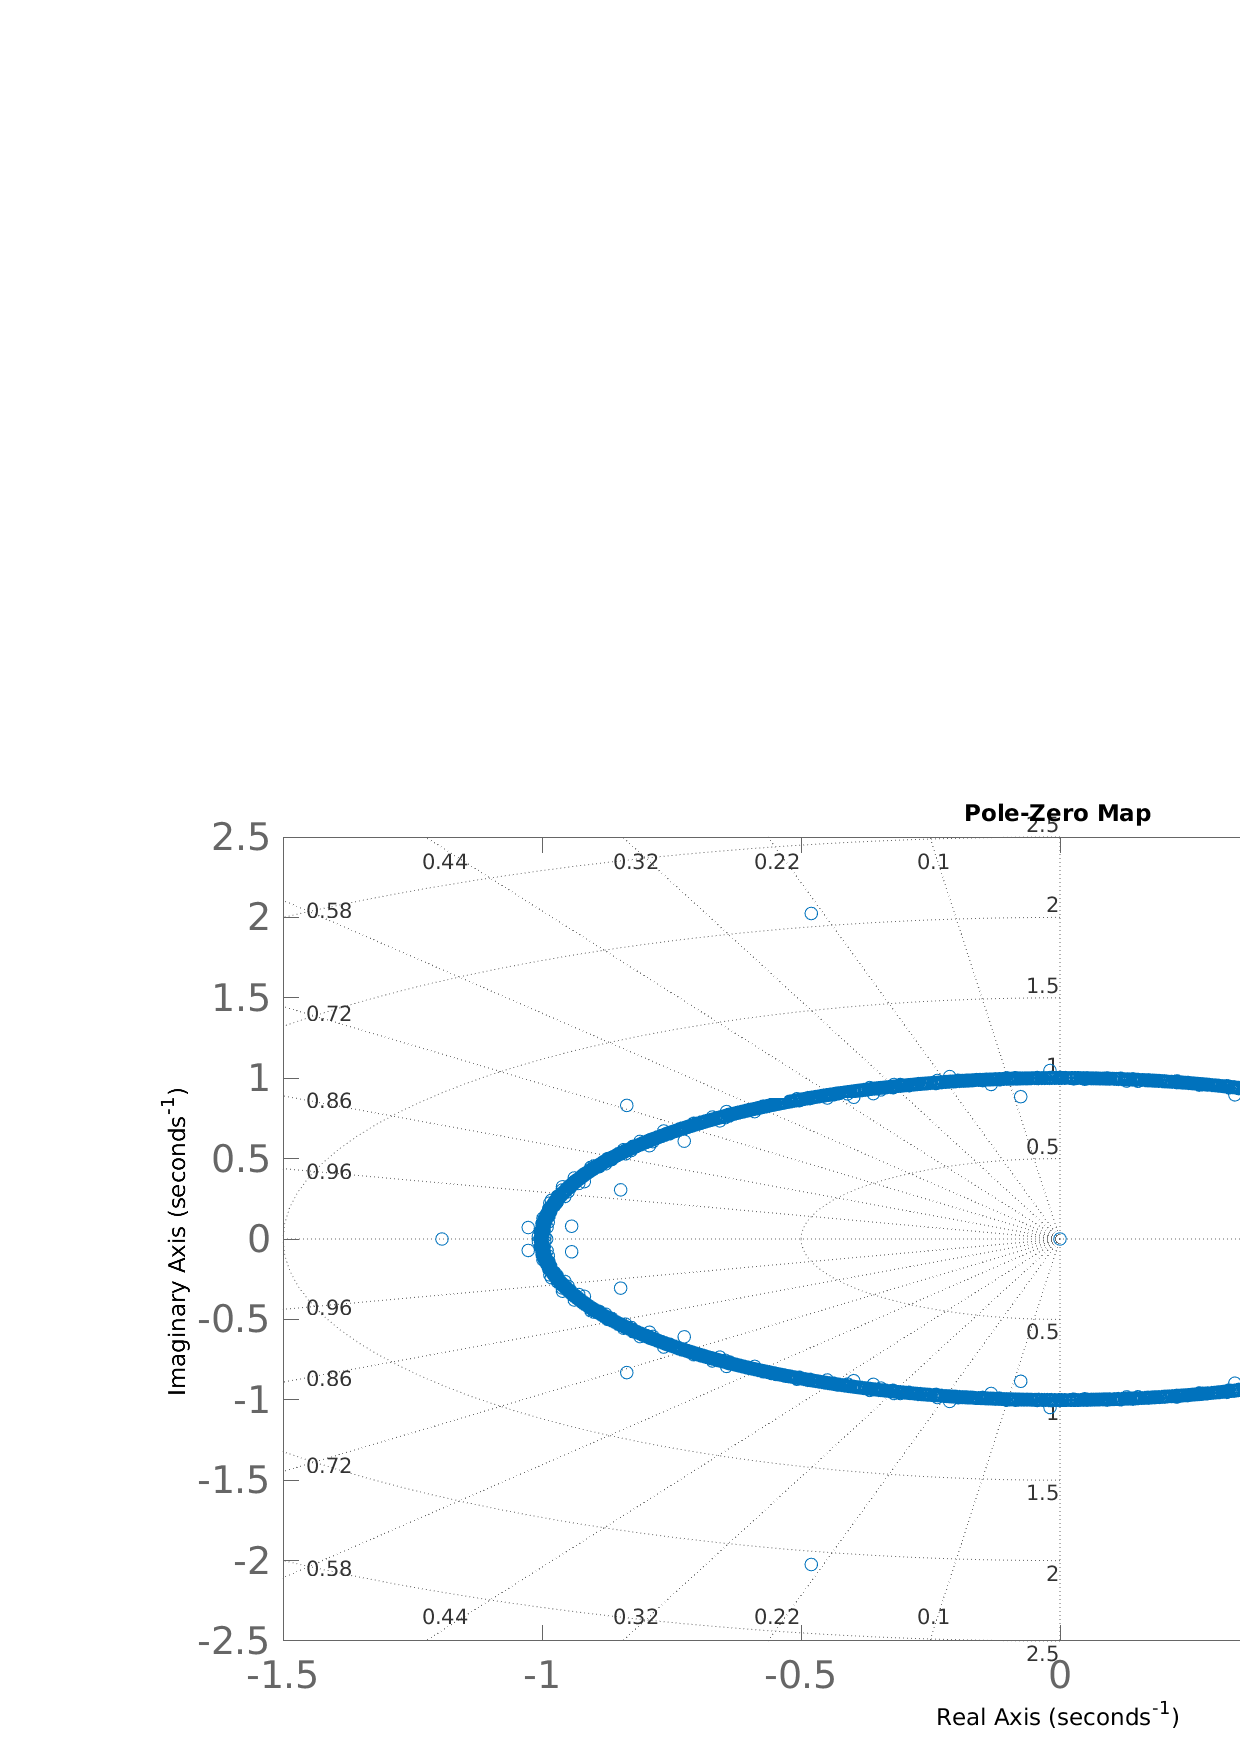
\includegraphics[width=\linewidth]{rir_pole_zero_plot.pdf}
\label{fig:rir_pole_zero}
\end{figure}

\subsection{Inverse filtering}
Inverse filtering is the most straight forward approach to compensate for the effects of reverberation. This approach depends on finding an inverse filter $g(n)$ such that it compensates the effects of RIR $h(n)$.
\begin{equation}
h(n)*g(n)=\alpha_i\delta(n-\tau_i)\text{,}
\label{eq:inv_filt}
\end{equation}
where $\alpha_i$ and $\tau_i$ represents arbitrary scaling and delay factor. This assumes that the RIR is known. The RIR can be estimated based on some methods discussed in Section~\ref{sec:inverse_fitering}. $g(n)$ can be obtained using the spectral analysis of (\ref{eq:inv_filt}). However, the direct application of inverse filtering is inappropriate because of the following reasons~\cite{naylor2010speech}. 
(i) the time-domain RIR is represented using thousands of coefficients. A similar number of coefficients are required to represent the inverse filter.  The estimation of such a high order system requires a robust algorithm with high numerical precision and computational cost. Further, even small errors in the RIR estimation (occurs especially in phase spectrum) can introduce a significant amount of artifacts in the estimated speech. In the presence of noise, the introduced artifacts will be more severe. 
(ii) The inverse filter is unstable as the RIR has a non-minimum phase response. 
(iii) The spectral nulls present in the RIR lead to strong peaks in the inverse filter. This leads to narrow-band noise amplification on the estimated dereverberated speech. 

The inverse filtering for multi-channel recordings is not as challenging as single-channel recording. For multi-channel recording of $M$ channels, utilizing MINT a set of stable inverse filters $g_m(n),m \in \{1,2,..,M\}$ can be obtained for the RIRs $h_m(n),m \in \{1,2,..,M\}$. Mathematically,
\begin{equation}
\sum_{m=1}^M h_m(n)*g_m(n) = \delta(n)\text{.}
\end{equation}
Various dereverberation methods based on MINT are discussed in Section~\ref{sec:MINT}.

As discussed previously, inverse filtering cannot be used for single-channel speech dereverberation. Singe-channel methods have to use various structures present in clean speech and RIR to perform speech dereverberation. Since the properties of clean speech and RIR (early part and reverberation tail) changes with time, short-time analysis is more fruitful. Short-time Fourier transform (STFT) and its variants are commonly used for this purpose. In this work various properties of magnitude STFT (magnitude spctrogram) of RIR is used. So, different properties of the RIR magnitude spectrogram is explained next.
\iffalse
\begin{itemize}
\item structure of RIR
\item early vs late part
\item non-minimum phase 
\begin{itemize}
\item single-channel RIR inversion is unstable
\item multi-channel inversion possible (MINT theorem)
\item need for STFT analysis - properties of speech, RIR used to enhance speech
\end{itemize}
\end{itemize}
\fi

\section{Magnitude spectrogram of RIR}
This section discusses the structure of a typical RIR magnitude spectrogram. The initial section discusses Polack's model which is a commonly used model for RIR. The later sections discuss different characteristics shown by a typical RIR.

\subsection{Pollack's model}
\label{sec:Pollacks_model}
Pollack's model for RIR is a time-domain model. The RIR is modeled as a non-stationary stochastic model~\cite{wen2008blind,kuttruff2016room}. The fine structure is statistically modeled as, 
\begin{equation}
h(n)=b(n)e^{-\tilde{\beta}n} \text{,}
\end{equation}
where $b(n)$ is a zero-mean stationary Gaussian random process with a power spectral density $B(k)$. $\tilde{\beta}$ is a damping factor that depends on the $T_{60}$. Based on the time-domain model, the frequency dependent energy envelope can be written as,
\begin{equation}
\mathbb{H}(k,n) = \mathbb{P}(k) e^{-2\beta(k)n}\text{,}
\end{equation}
where $\mathbb{P}(k)$ represents the spectral envelope. It represents the spectrum of the frame that contains maximum energy (in this case $\mathbb{H}(k,0)$). The damping factor $\beta(k)$ depends on $T_{60}$ as shown in (\ref{eq:RT60}). 
\begin{equation}
\beta (k)= \dfrac{3\text{ln}(10)}{T_{60}(k) f_s}\text{,}
\label{eq:RT60}
\end{equation}
where $f_s$ represents the sampling frequency. The $T_{60}$ (hence $\beta (k)$) changes with frequency~\cite{jeub2010we}. The variation of $T_{60}(k)$ with frequency $k$ is small for certain RIRs while for others the variation is large. 
The RIR magnitude spectrogram for the model can be approximated as,
\begin{equation}
H(k,n)\approx P(k) e^{- \beta(k) n},
\label{eq:PollackModel}
\end{equation} 
where $P(k)$ represents the spectral envelope ($H(k,0)$). 

\iffalse
%where, $P(k)$ represents the initial spectrum 
and $\beta(k)$ is related to the reverberation time ($T_{60}$) of the RIR as shown in (\ref{eq:RT60}). The $T_{60}$ (hence $\delta (k)$) changes with frequency~\cite{jeub2010we}. The variation of $T_{60}(k)$ with frequency $k$ is small for certain RIRs while for others the variation is large.

A model for the time-frequency variation for RIR spectrogram is discussed in \cite{wen2008blind,kuttruff2016room}. The model is based on Pollack's model for RIR. The RIR spectrogram for the model can be approximated as,
\begin{equation}
H(k,n)\approx P(k) e^{-2 \delta(k) n},
\label{eq:PollackModel}
\end{equation} 
where $P(k)$ represents the magnitude spectrum of the first frame of the RIR spectrogram ($H(k,0)$) 
%where, $P(k)$ represents the initial spectrum 
and $\delta(k)$ is related to the reverberation time ($T_{60}$) of the RIR as shown in (\ref{eq:RT60}). The $T_{60}$ (hence $\delta (k)$) changes with frequency~\cite{jeub2010we}. The variation of $T_{60}(k)$ with frequency $k$ is small for certain RIRs while for other the variation is large.  
\begin{equation}
\beta (k)= \dfrac{3\text{ln}(10)}{T_{60}(k) f_s},
\label{eq:RT60}
\end{equation}
where $f_s$ is the sampling frequency. Figure~\ref{fig:RIR_spectrogram} shows the magnitude spectrogram of a measured RIR. It can be observed that the RIR spectrogram has a frequency envelope which decays with time as predicted in (\ref{eq:RT60}). The rate of decay changes with frequency. Also, most of the variations occur during the initial few frames after the direct path. The RIR spectrogram obtained based on the proposed RIR model shown in Figure~\ref{fig:RIR_approx} also incorporates these properties about RIR spectrogram.  A similar observations were obtained for other measured RIRs. This observation justifies the use of the proposed RIR spectrograms model. 
\begin{figure}
\centering
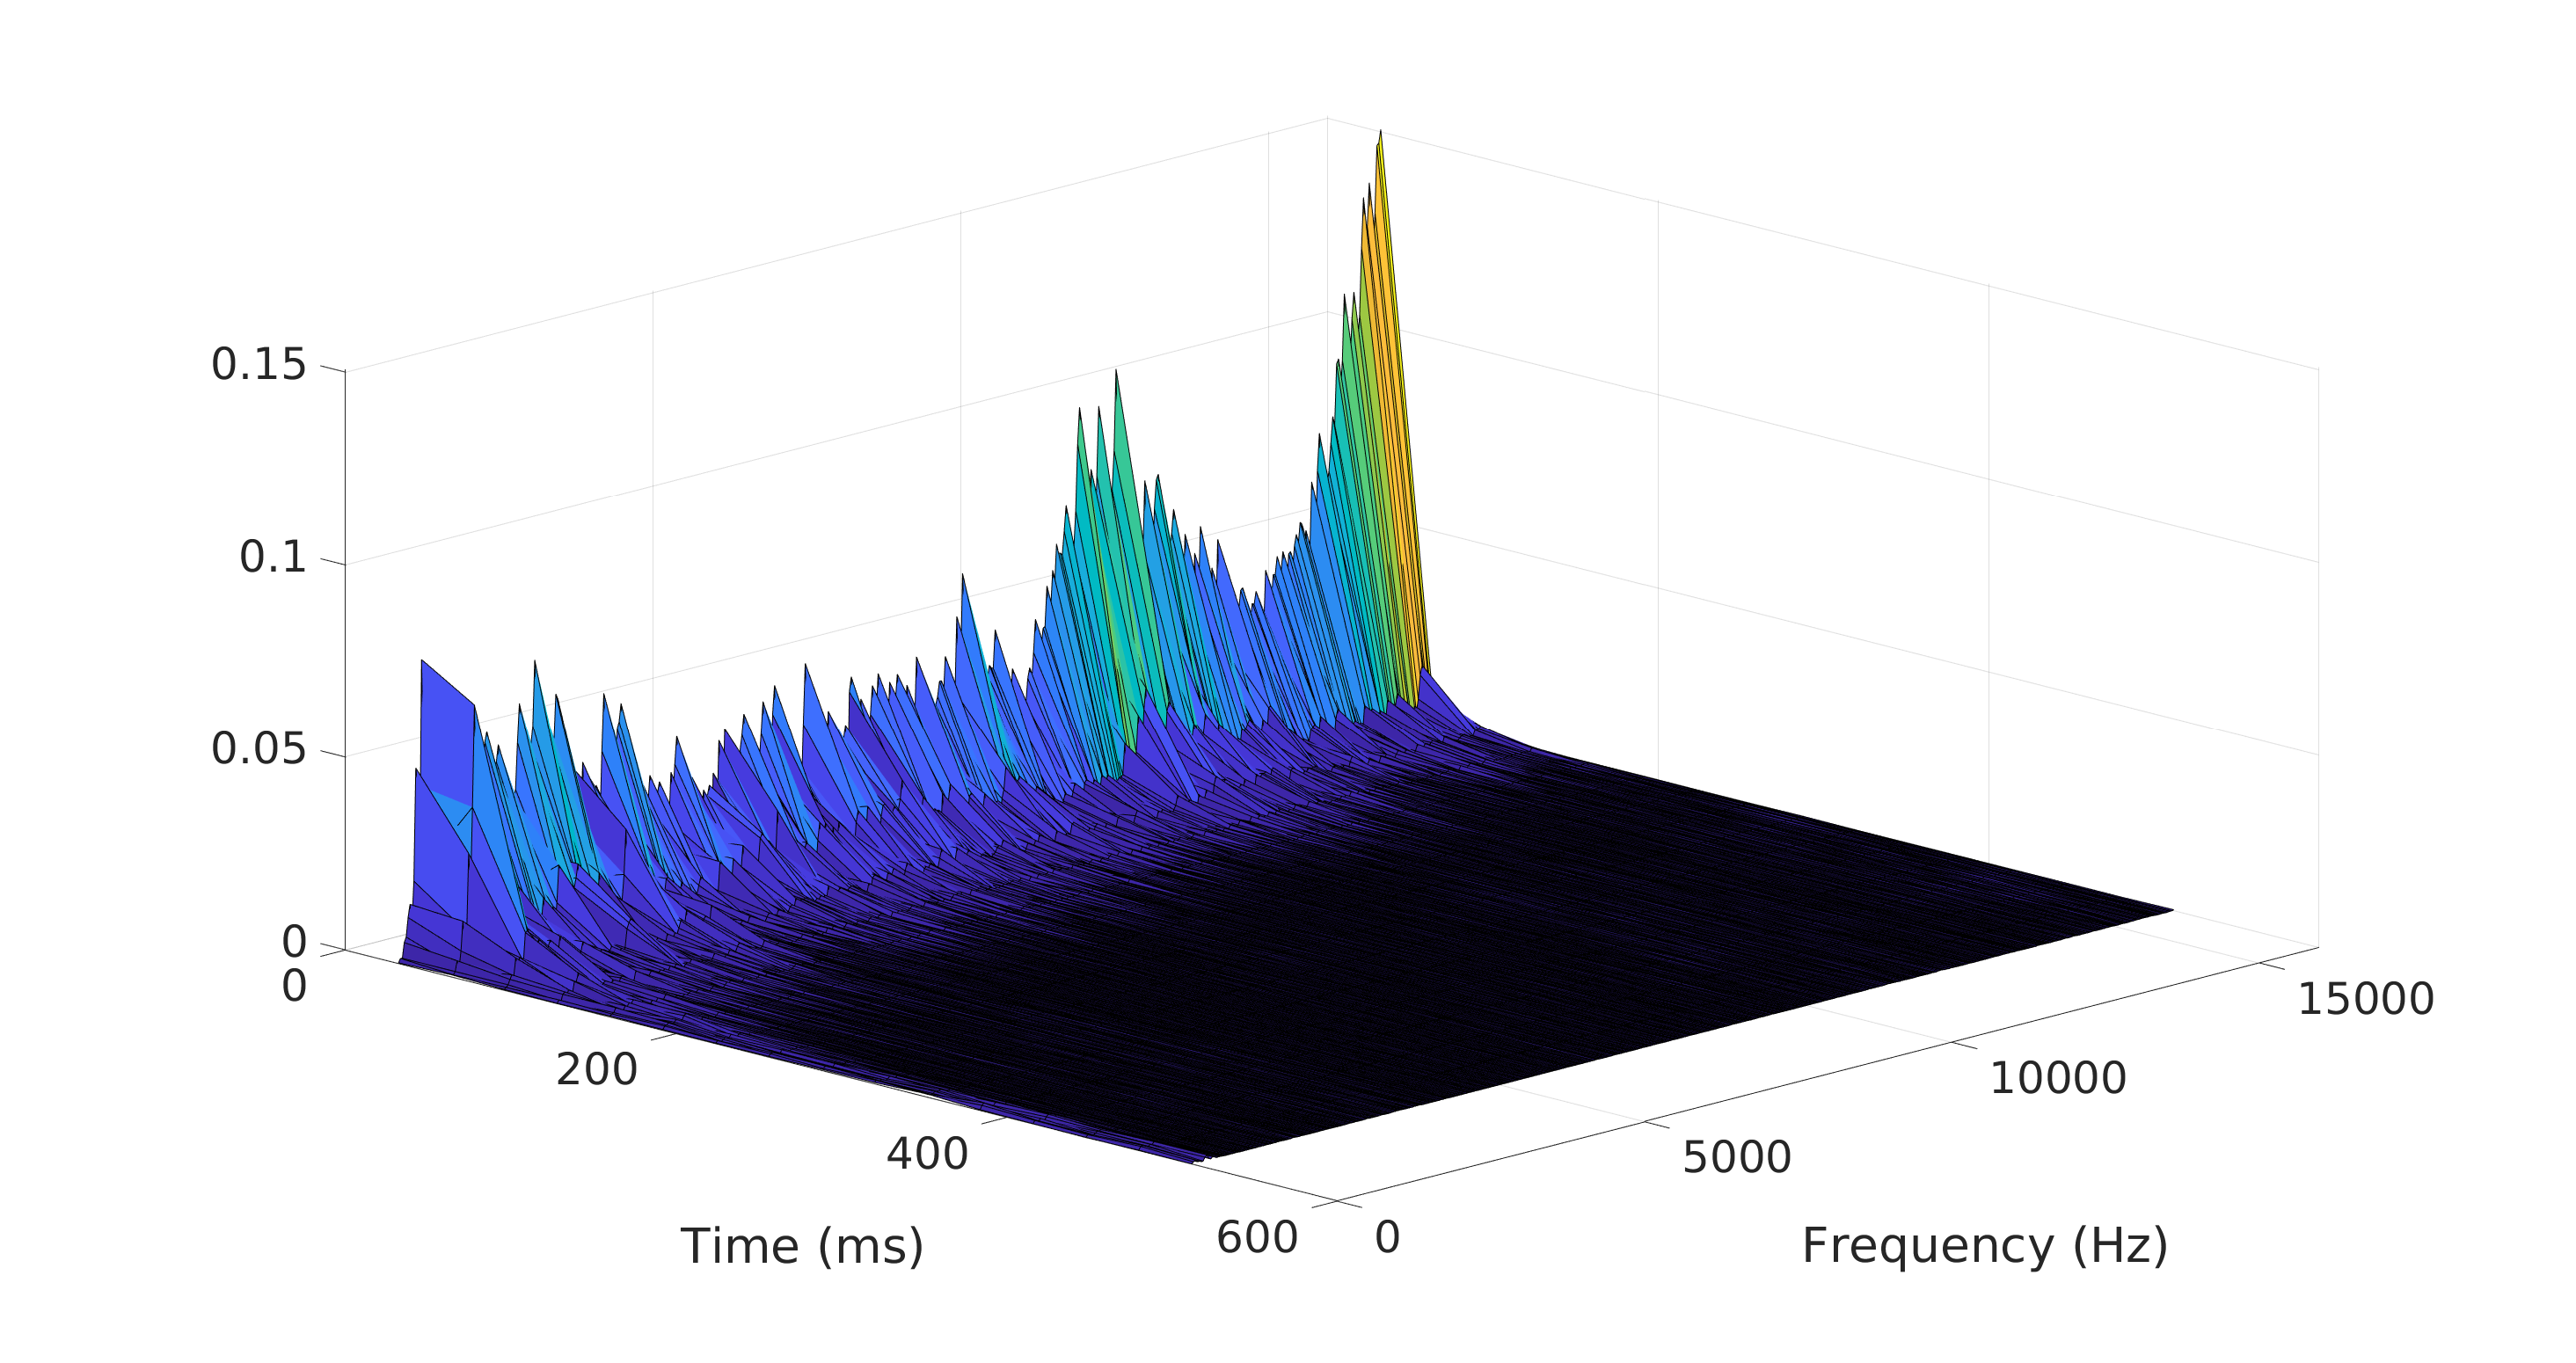
\includegraphics[width=\linewidth]{fig/RIR_original.eps}
\caption{RIR spectrogram obtained for a measured RIR. The RIR has an approximate $T_{60}$ of $500$~ms and source-to-microphone distance (d) of $0.5$~m.}
\label{fig:RIR_spectrogram}
\end{figure}
\fi

\subsection{Spectrogram structure of RIR}
This section details the time-frequency structure present in RIR magnitude spectrogram. The results of the analysis was shown for a particular RIR. However, a similar observations were obtained for other RIRs. 

\subsubsection{Spectral and temporal variations}
This section discusses the frequency envelope and temporal variation of an RIR magnitude spectrogram. The frequency envelope is represented as the spectrum of the frame of RIR having maximum energy. The temporal envelope for a frequency bin $k=\kappa$ represents the variation of RIR spectrogram with time $n$ for a fixed frequency bin i.e, $H(\kappa, n)\text{, }n\in\{0,1,...(L_h-1)\}$.

Figure~\ref{fig:RIR_spectrogram} represents the frequency envelope and temporal variation for different frequency bands for a measured RIR is shown. The RIR has a $T_{60}\approx 700$~ms and a source-microphone distance of $2$~m. It is obtained from REVERB challenge RIR~\cite{kinoshita2016summary}.  Most of the energy in the temporal envelope is concentrated in the initial few frames. The temporal envelope for different frequency bands is shown to decay with time. The decay rate changes with frequency. However, the decays are not strictly exponential as predicted in Pollack's model in Section~\ref{sec:Pollacks_model}. But the model gives a good insight into the time-frequency structure of the magnitude spectrogram of RIR.
\begin{figure}
\centering
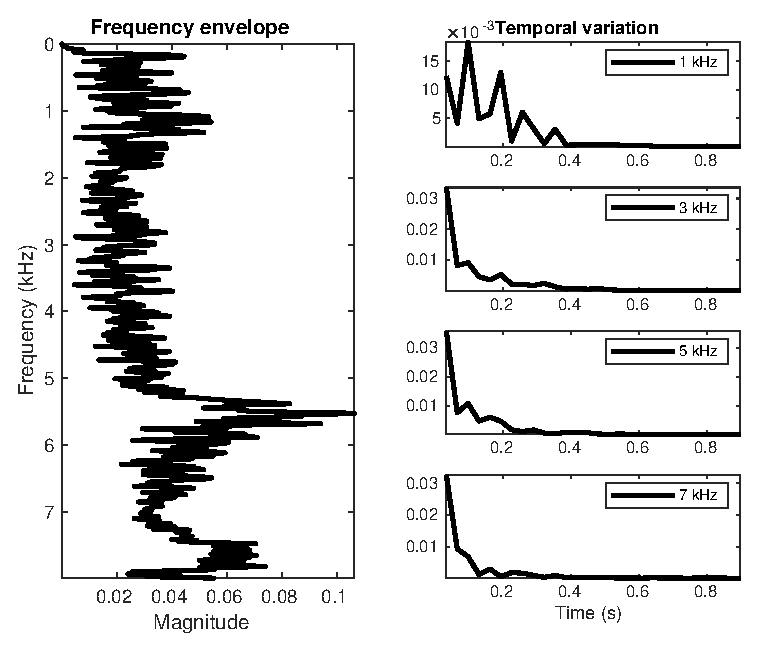
\includegraphics[width = \linewidth]{fig/RIR_Rank1_Original.eps}
\caption{The magnitude spectrogram (left) and temporal envelope for different frequency bands (right) for a measured RIR with $T_{60}\approx700$~ms and source-microphone distance of $2$~m. The temporal envelope decays down with time as is the case in Pollack's model. }
\label{fig:RIR_spectrogram}
\end{figure}

\subsubsection{Sparsity}
Figure~\ref{fig:RIR_spectrogram} shows the spectral envelope and temporal variation of a measured RIR.  It is observed that for all frequency bands, most of the high energy regions occur during the initial few frames after the direct path and dies down to zero after a few frames. This results in the RIR spectrogram having near-zero values for the later frames. In other words, it can be said that the RIR spectrogram is sparse. 

\subsubsection{Separability assumption}
\label{sec:Separability_assumption}
As explained earlier sections, the RIR specrtogram has frequency and time structures. One of the most simplest approach is to treat the temporal and spectral variations independently~\cite{mohanan201a}. The RIR spectrogram $\mathbf{H}$ can be represented with a frequency envelope $H_1(k)$ and temporal variation $H_2(n)$. Mathematically,
\begin{align}
H(k,n) &\approx H_1(k)H_2(n) \text{,}
\end{align}
A rank-$1$ NMF decomposition is performed on the RIR magnitude spectrogram $\mathbf{H}$ to obtain an estimate for $H_1(k)$ and $H_2(n)$. NMF is an iterative algorithm based on a cost function~\cite{lee99}. The cost function is used to measure the correctness of the RIR magnitude spectrogram estimate with the original RIR magnitude spectrogram. In this work, generalized Kullback-Leibler (KL) divergence is used as the cost function. The cost function is represented as,   
\begin{align}
C_{SA} &= \sum_{k = 0}^{K-1}\sum_{n=0}^{L_h-1}\text{KL} (H(k,n)|\hat{H}_{sep}(k,n)) \nonumber \\
\text{KL}(u|v) &= u\text{ln}(\dfrac{u}{v}) + v - u,
\label{eq:KLdiv}
\end{align} 
where $\hat{H}_{sep}(k,n)=H_1(k)H_2(n)$ represents the rank-$1$ approximation of the RIR spectrogram.  A rank-$1$ approximation for the Pollacks model shown in (\ref{eq:PollackModel}) can be obtained by assuming $T_{60}$ is independent of frequency. For this case, $H_1(k) = P(k)$ and $H_2(n)=e^{-\beta n}$.

Figure~\ref{fig:RIR_rank_1_spectrogram} compares the frequency envelope and temporal variation of rank-$1$ approximated RIR spectrogram with the original RIR magnitude spectrogram. It can be observed that most variations of frequency envelope are captured using rank-$1$ approximated  RIR spectrogram. However, the approximation of temporal variations does not capture most of the variations. The main reason for this that the temporal variation changes with frequency band $\kappa$. However, in rank-$1$ approximated RIR magnitude spectrogram model the temporal variation is the same except for a scaling factor of $H_1(\kappa)$. This can pose a limitation in accurately representing the RIR spectrogram.   

\begin{figure*}[ht]
\begin{tabular}{cc}
\subfloat[]{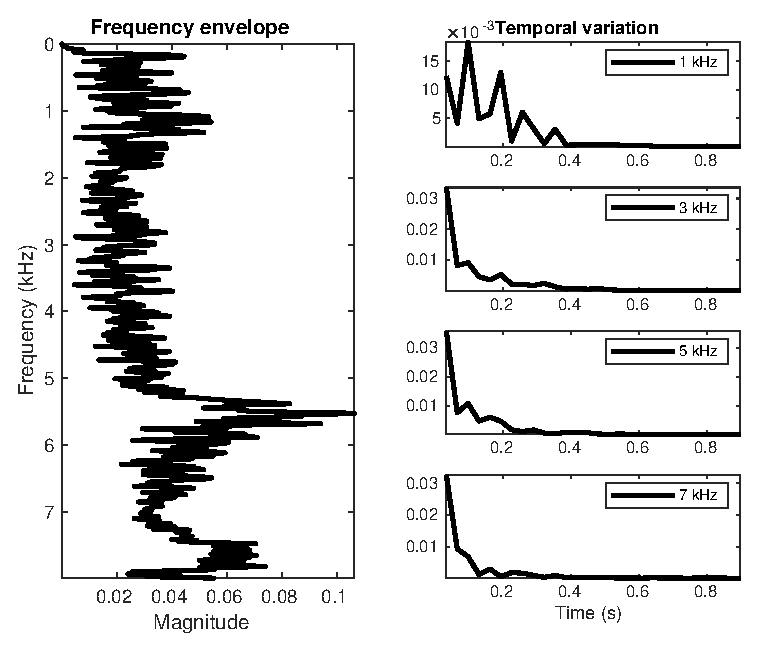
\includegraphics[width = 0.5\linewidth]{fig/RIR_Rank1_Original.eps}} &
\subfloat[]{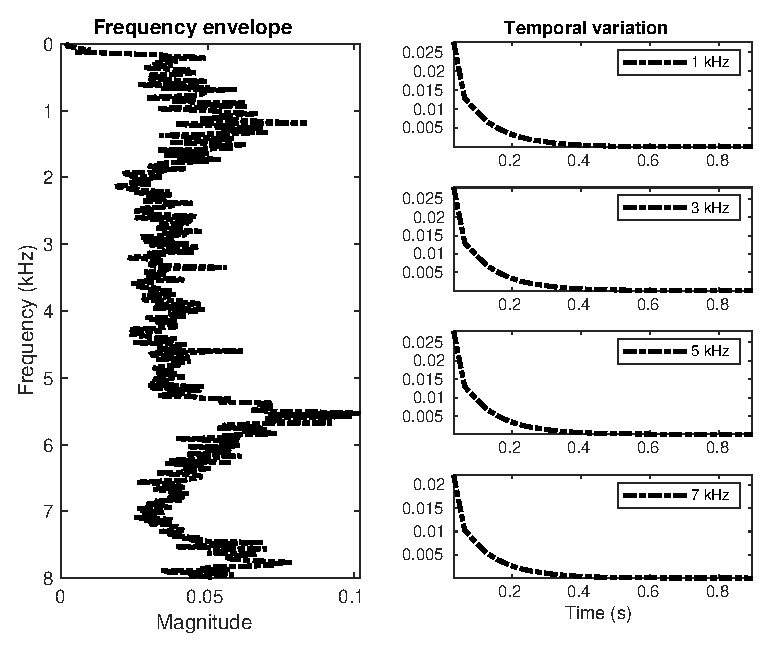
\includegraphics[width = 0.5\linewidth]{fig/RIR_Rank1_Approx.eps}}\\
\end{tabular}
\caption{(a) Frequency envelope and temporal variation obtained for a measured RIR from~\cite{kinoshita2016summary} with $T_{60}\approx 700$~ms and source-to-microphone distance $d=2$~m. (b) Frequency envelope and temporal variation obtained by a rank-$1$ NMF decomposition of the RIR. Frequency envelope approximated in (b) captures the most variations in (a).}
\label{fig:RIR_rank_1_spectrogram}
\end{figure*}
%Such an approximation is a very crude representation of RIR magnitude spectrogram. In this model the temporal variations $H_2(n)$ is assumed to be independent of frequency $k$. One of the imitations of this model is it cannot model the frequency dependency of $T_{60}$. 

\subsubsection{Low-rank nature}
As discussed in Section~\ref{sec:Separability_assumption}, the separability approximation for the RIR magnitude spectrogram is inaccurate. A low-rank approximation is a better model. Based on the low-rank approximation, RIR magnitude spectrogram $\mathbf{H}$ can be represented as,
\begin{align}
\mathbf{H} &\approx \mathbf{H}_1\mathbf{H}_2 \text{,}
\end{align}
where, $\mathbf{H}_1 \in \mathbb{R}_+^{K \times P}$ and $\mathbf{H}_2 \in \mathbb{R}_+^{P \times L_h}$ represents the bases and activation matrix for the NMF decomposition, respectively. $P$ represents the rank of NMF decomposition. Low-rank approximation results in reducing the number of parameters used to represent the RIR spectrogram from $KL_h$ to $P(K+L_h)$~\footnote{$P$ in this case is selected such that $P<L_h$ and $P<<K$}.
$\mathbf{H}_1$ contains $P$ set of frequency envelopes $\mathbf{H}_1^{(p)}\in \mathbb{R}_+^{K \times 1} \text{, } p\in \{1,2,...,P \}$ and $\mathbf{H}_2$ contains the corresponding $P$ set temporal variations $\mathbf{H}_2^{(p)}\in \mathbb{R}_+^{1 \times L_h} \text{, } p\in \{1,2,...,P \}$. Mathematically,
\begin{align}
\mathbf{H}_1 &= \bigg[\mathbf{H}_1^{(1)}\bigg|\mathbf{H}_1^{(2)}\bigg|...\bigg|\mathbf{H}_1^{(P)}\bigg] \nonumber \\
\mathbf{H}_2 &= \bigg[\mathbf{H}_2^{(1)^T}\bigg|\mathbf{H}_2^{(2)^T}\bigg|...\bigg|\mathbf{H}_2^{(P)^T} \bigg]^T
\end{align}
$\mathbf{H}_1$ and $\mathbf{H}_2$ are obtained by performing a NMF decomposition on RIR magnitude spectrogram $\mathbf{H}$.

There exist different approaches to obtain a low-rank approximation. However, the use of NMF decomposition is preferred for the following reason. It ensures that the low-rank approximated RIR spectrogram is non-negative. This is a necessary condition for using a low-rank model in reverberation model discussed in Section~\ref{sec:NMF_methods}. Further, imposing the non-negative constraint on $\mathbf{H}_1$ and $\mathbf{H}_2$ does not compromise on the quality of the estimates as discussed next. 

The cost function used for the purpose has structure similar to (\ref{eq:KLdiv}). The cost function $C_H$ for the purpose can be written as,
\begin{align}
C_{H} &= \sum_{k = 0}^{K-1}\sum_{n=0}^{L_h-1}\text{KL} (H(k,n)|\hat{H}_{rank-P}(k,n)) \nonumber \\
\hat{H}_{rank-P}(k,n) &= \sum_{p=1}^P H_1^{(p)}(k) H_2^{(p)}(n)
\end{align}
where $\hat{H}(k,n)$ is the  (k,n)-th element of the low-rank approximated RIR spectrogram. $H_1^{(p)}(k)$ and $H_2^{(p)}(n)$ represents the elements of $\mathbf{H}_1^{(p)}$ and $\mathbf{H}_2^{(p)}$, respectively.


\iffalse
Experimentally it can be shown that the low-rank approximated RIR spectrogram $\mathbf{\hat{H}}$ is a good approximation for the original RIR spectrogram. A low-rank RIR spectrogram is obtained using a multiplicative algorithm proposed in~\cite{lee99}. It uses Generalized Kullback-Leibler (KL) divergence as the cost function. The cost function used in the work are summarized as,
\begin{align}
C_{rank-P} &= \sum_{k = 0}^{K-1}\sum_{n=0}^{L_h-1}\text{KL} (H(k,n)|\hat{H}(k,n)) \nonumber \\
\text{KL}(u|v) &= u\text{log}(\dfrac{u}{v}) + v - u,
\label{eq:KLdiv1}
\end{align} 
where $\hat{H}(k,n)$ is the  (k,n)-th element of the low-rank approximated RIR spectrogram.
\fi
 
$C_{H}$ captures the net deviation occurred due to the low-rank approximation of the RIR spectrogram. The deviation $C_{H}$ depends on the rank-$P$ of the decomposition. Figure~\ref{fig:cost_rank_P_approximation} analyses this dependency for different measured RIR available from~\cite{kinoshita2016summary}. The figure shows the mean and extreme variation for $C_{H}$ with $P$. It is observed that deviation reduces with increasing $P$, and variation saturates after $P=10$ indicating that a rank-$P$ approximation is sufficient for the purpose. 
Figure~\ref{fig:RIR_rank_P_spectrogram} compares the original frequency envelope and temporal variation of a RIR with the one obtained using a rank-$10$ NMF decomposition. The frequency envelope and temporal variation present in the original RIR magnitude spectrogram is accurately captured using a rank-$10$ approximation.
\begin{figure}[ht]
\centering
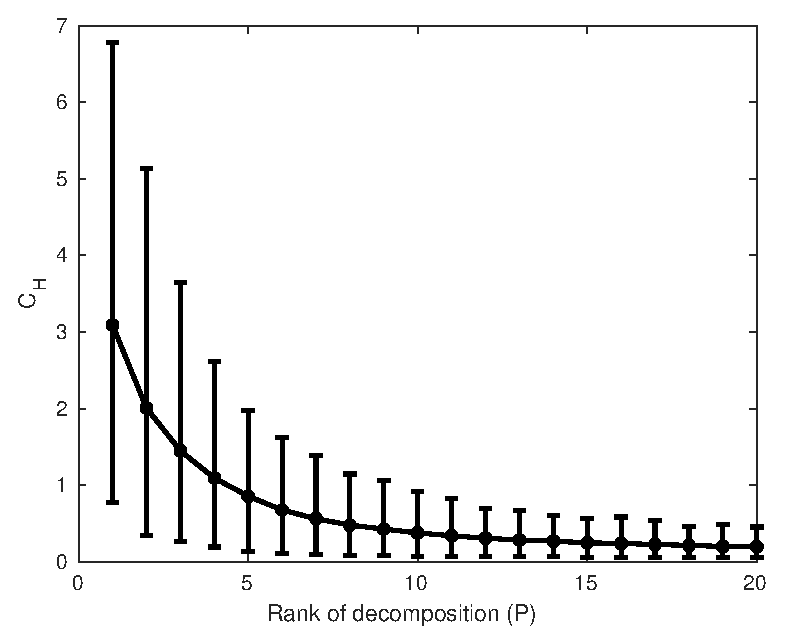
\includegraphics[width=\linewidth]{fig/RIR_NMF_approx_cost_error_plot.eps}
\caption{Effect of varying rank $P$ on the low-rank approximation for the RIR spectrogram. The deviation from the original RIR spectrogram reduces with increasing $P$. The deviation is small for $P>10$.}
\label{fig:cost_rank_P_approximation}
\end{figure}

\begin{figure*}[ht]
\begin{tabular}{cc}
\subfloat[]{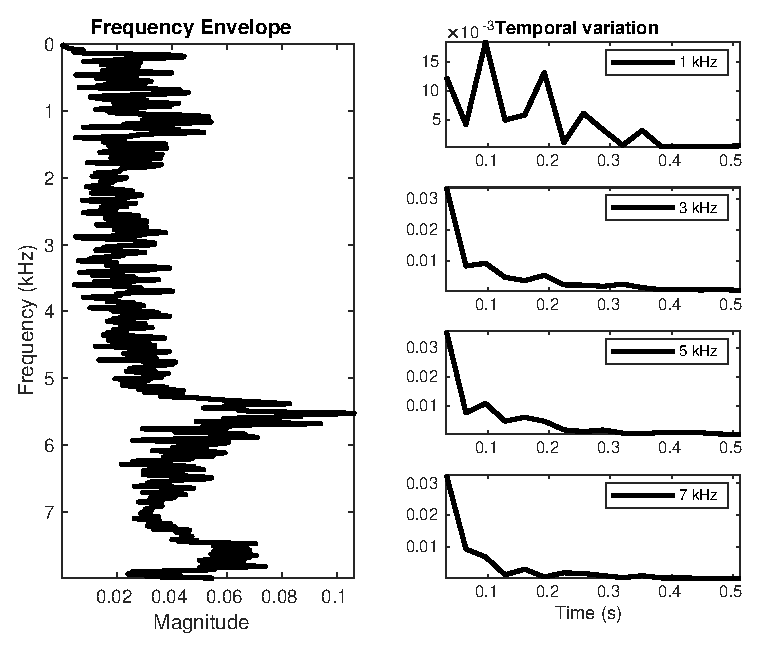
\includegraphics[width = 0.5\linewidth]{fig/RIR_NMF_far_original.eps}} &
\subfloat[]{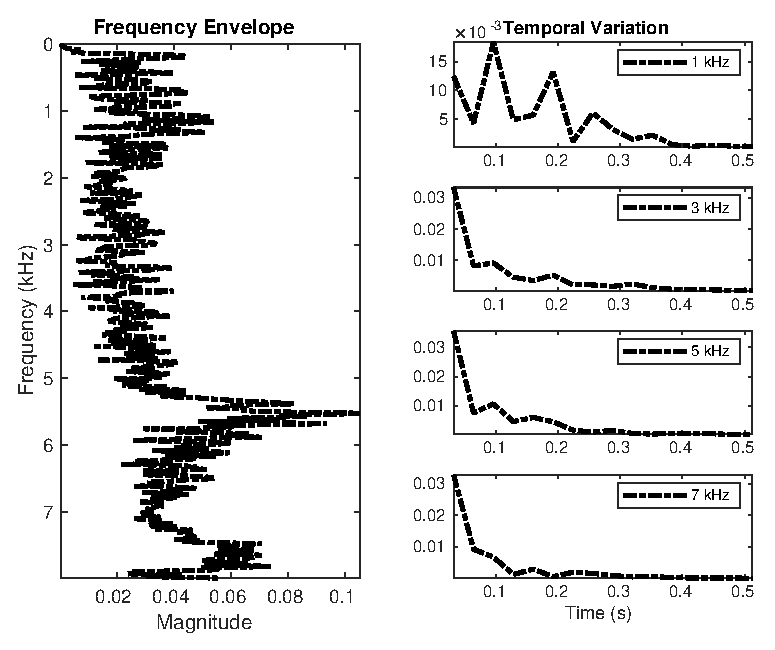
\includegraphics[width = 0.5\linewidth]{fig/RIR_NMF_far_approx.eps}}\\
\end{tabular}
\caption{(a) Frequency envelope and temporal variation obtained for a measured RIR from~\cite{kinoshita2016summary}. (b) Frequency envelope and temporal variation obtained by a rank-$10$ NMF decomposition of the RIR. (b) is a very good approximation of (a).}
\label{fig:RIR_rank_P_spectrogram}
\end{figure*}

\iffalse
\begin{figure*}[ht]
\begin{tabular}{cccc}
\subfloat[]{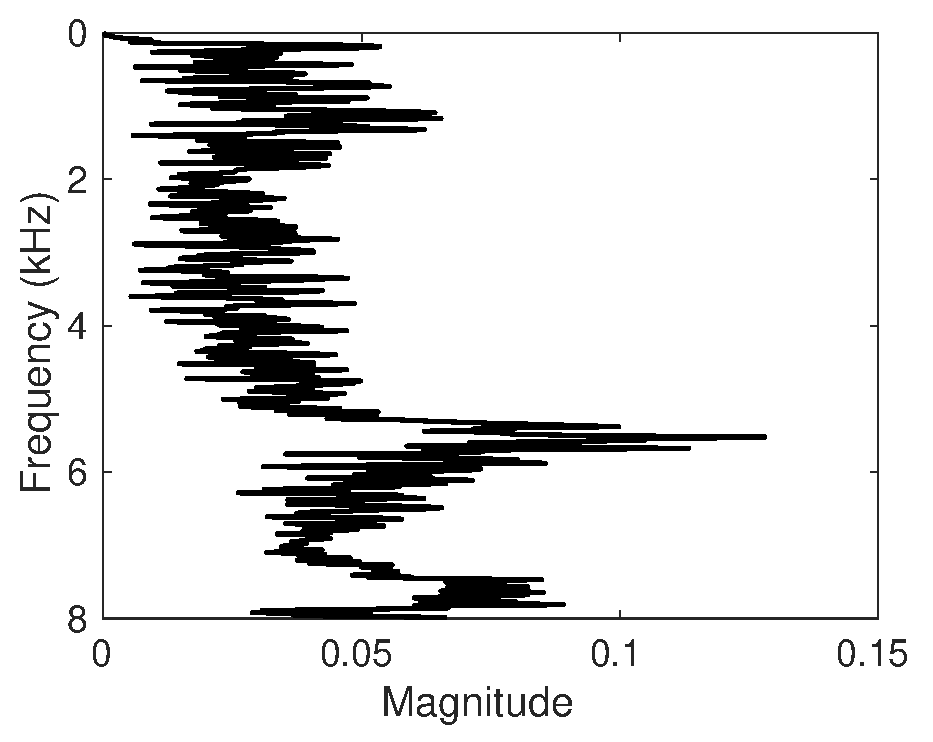
\includegraphics[width = 0.25\linewidth]{fig/RIR_env_original_RIR_cond_RIR_SimRoom3_far_AnglA_StationaryNoise_10dB.eps}} &
\subfloat[]{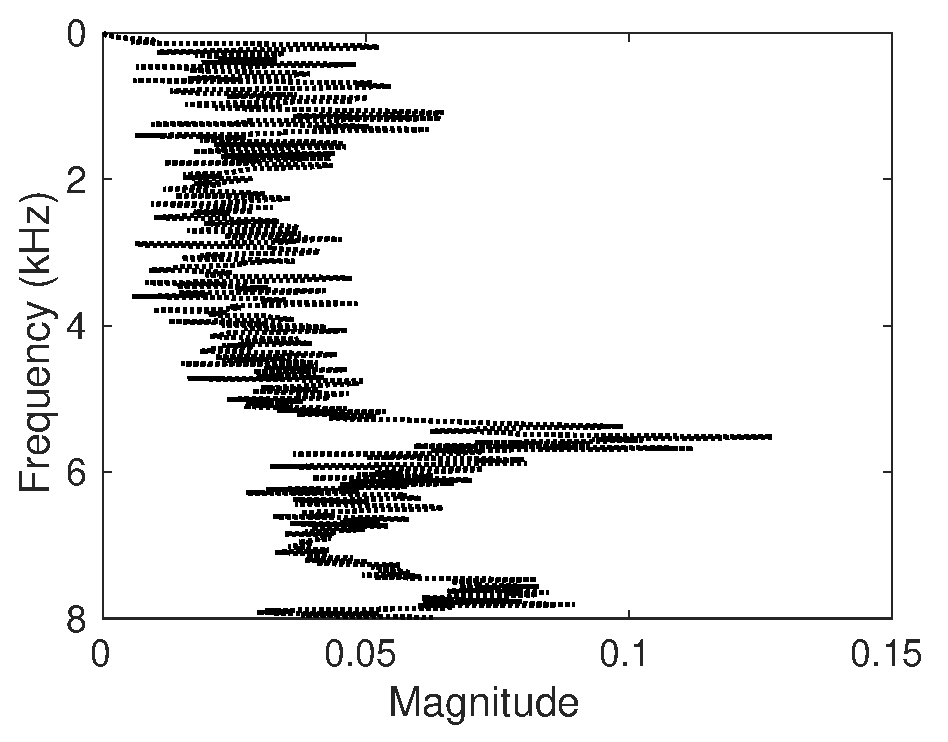
\includegraphics[width = 0.25\linewidth]{fig/RIR_env_approx_RIR_cond_RIR_SimRoom3_far_AnglA_StationaryNoise_10dB.eps}} &
\subfloat[]{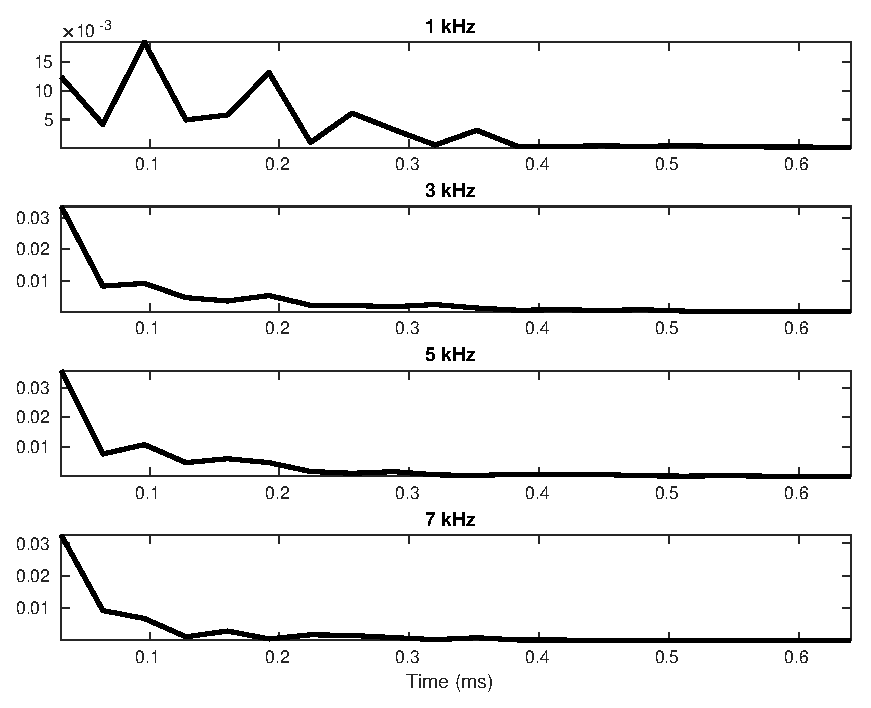
\includegraphics[width = 0.25\linewidth]{fig/RIR_tempo_original_RIR_cond_RIR_SimRoom3_far_AnglA_StationaryNoise_10dB.eps}} &
\subfloat[]{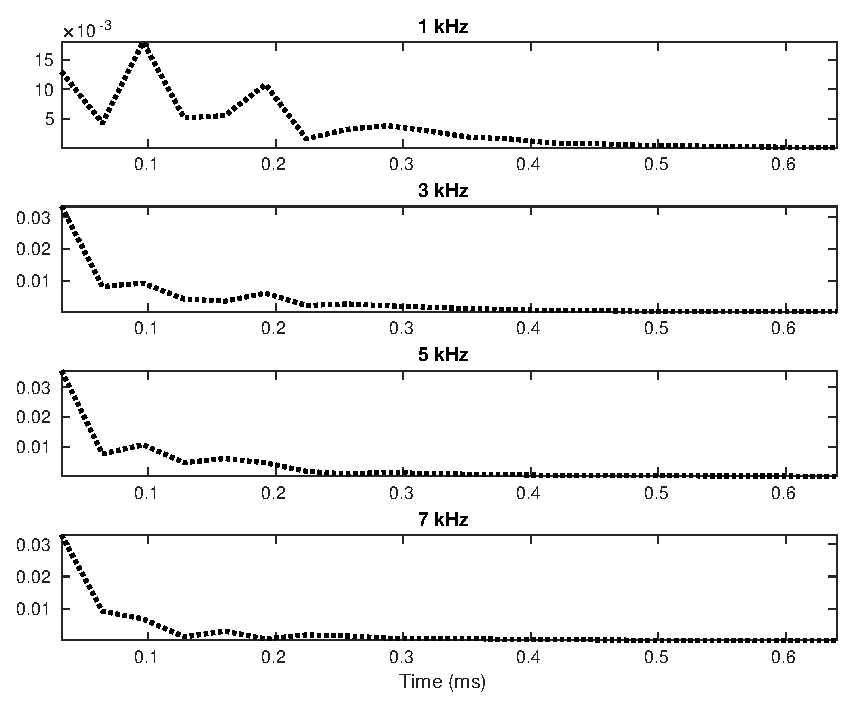
\includegraphics[width = 0.25\linewidth]{fig/RIR_tempo_approx_RIR_cond_RIR_SimRoom3_far_AnglA_StationaryNoise_10dB.eps}} \\
\end{tabular}
\caption[abc]{(a) Frequency envelope and temporal variation for different bands for the spectrogram obtained for a measured RIR from~\cite{kinoshita2016summary} having an approximate $T_{60}$ of $500$~ms and source-to-microphone distance (d) of $2$~m. (b) Frequency envelope and temporal variation obtained by a rank-$10$ NMF decomposition of the RIR. (b) is a very good approximation of (a).}
\label{fig:RIR_rank_P_spectrogram}
\end{figure*}
\fi

\section{Characteristics of RIR}
This Section details the various parameters associated with a RIR. 

\subsection{Source-microphone distance ($d_{sd}$)}
The structure of RIR changes with the position of microphone and source, especially the source-microphone distance ($d_{sm}$). The direct-path energy decreases with an increase in $d_{sm}$, whereas the diffused nature of reverberation results in the reverberant energy remaining mostly constant~\cite{naylor2010speech}. As a result, the effects due to the reverberation tail becomes more prominent with increasing distance.

\subsection{Reverberation time ($T_{60}$)}
When a sound source placed in a reverberant room is switched off, it takes a finite time for the sound level to decay down. The $T_{60}$ is defined as the time taken for the sound level to drop $60$~dB below the level at sound cessation~\cite{ratnam2003blind}. $T_{60}$ is fixed of a reverberant room. Typically, $T_{60}$ varies with properties of the room like absorption coefficients of the wall, etc and is independent of the position of source and microphone~\cite{naylor2010speech}. Reverberation time changes with frequency~\cite{jeub2010we}, but it is typically represented by a single value which indicates the dominant mode~\cite{naylor2010speech}.  

\subsection{Direct-to-reverberation ratio (DRR)}
DRR is defined as the ratio of energy present in the direct-path and early reflections of the RIR to the total energy present in the RIR~\cite{kinoshita2016summary}. The reflections delayed upto  $50$~ms from the direct-path forms the early part. Mathematically,
\begin{align}
DRR &= \dfrac{\sum_{n=0}^{n_e}h^2(n)}{\sum_{n=n_e+1}^{L_h} h^2(n)} \nonumber \\
\dfrac{n_e}{f_s}  &= 50\times 10^{-3} \text{s,}
\end{align} 
where $n_e$ represents the number of samples used to represent the early part of RIR. $f_s$ represents the sampling frequency. DRR gives a measure of the contribution of coloration occurring due to the early part of RIR to the net effects of reverberation. DRR varies with $d_{sm}$ and $T_{60}$~\cite{naylor2010speech}.

\section{Conclusion}
This chapter discussed the various time and frequency domain structure present in RIR. The disadvantage of using single-channel inverse filtering approaches was discussed next. Finally, different structures present in the magnitude spectrogram of RIR is discussed. The following chapters will utilize these RIR spectrogram structures in the speech enhancement algorithms.